\documentclass[tikz]{standalone}

\colorlet{FilledSurface}{blue!20}
\colorlet{FilledSurfaceGroupOne}{blue!20}
\colorlet{FilledSurfaceGroupTwo}{red!20}
\colorlet{FilledSurfaceGroupThree}{green!20}
\colorlet{FilledSurfaceGroupFour}{magenta!20}
\colorlet{FormulaBackground}{green!10}
\colorlet{FormulaFrame}{green}


\usetikzlibrary{calc, angles}

\begin{document}
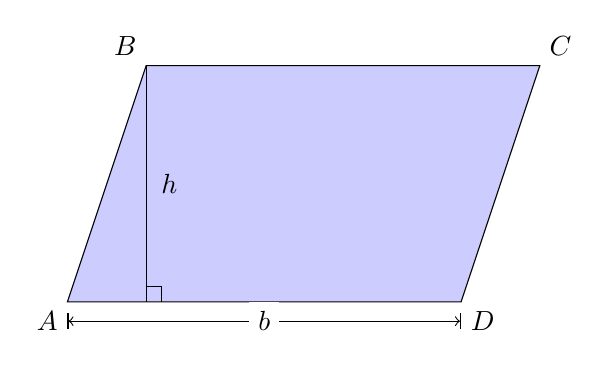
\begin{tikzpicture}

\coordinate (A) at (0, 0);
\coordinate (B) at (1, 3);
\coordinate (C) at (6, 3);
\coordinate (D) at (5, 0);
\draw[fill = FilledSurfaceGroupOne]
    (A) node[below left]{$A$}
    -- (B) node[above left]{$B$}
    -- (C) node[above right]{$C$}
    -- (D) node[below right]{$D$}
    -- cycle;

\coordinate (H) at (B |- A);

\draw[color = black,|<->|] ($(A)!7pt!-90:(D)$) to node [fill=white, midway] {$b$} ($(D)!7pt!90:(A)$);
\draw (B) -- node [right=2pt] {$h$} (H);
\path pic [draw,angle radius=2mm] {right angle = B--H--D};

\end{tikzpicture}
\end{document}


